\documentclass[11pt,a4paper]{article}

\usepackage[margin=1.8cm,footskip=0.9cm]{geometry}
\usepackage[T1]{fontenc}
\usepackage{lmodern}
\usepackage{microtype}
\usepackage{xcolor}
\usepackage{graphicx}
\usepackage{enumitem}
\usepackage{tabularx}
\usepackage{ragged2e}
\usepackage{needspace}
\usepackage{fancyhdr}
\usepackage{hyperref}

\hypersetup{hidelinks,pdftitle={Curriculum Vitae},pdfauthor={Nathan Wallheimer}}
\urlstyle{same}

\pagestyle{fancy}
\fancyhf{}
\fancyfoot[L]{\small\color{gray}Nathan Wallheimer\enspace|\enspace Curriculum Vitae}
\fancyfoot[R]{\small\color{gray}\thepage}
\renewcommand{\headrulewidth}{0pt}

\newcommand{\cvsection}[1]{%
  \par\addvspace{1.1\baselineskip}\Needspace{4\baselineskip}%
  {\large\bfseries #1\par}\nobreak\vspace{3pt}%
  {\color{gray}\hrule height 0.4pt}\nobreak\vspace{6pt}}
\newcommand{\datedentry}[2]{%
  \begin{tabularx}{\textwidth}{@{}p{2.7cm}@{\hspace{0.3cm}}>{\RaggedRight\arraybackslash}X@{}}
    #1 & #2
  \end{tabularx}\par\smallskip}
\newcommand{\doi}[1]{\mbox{\href{https://doi.org/#1}{\nolinkurl{doi:#1}}}}
\newcommand{\publication}[3]{%
  \item \begin{minipage}[t]{\linewidth}
    \RaggedRight #2\par\vspace{1pt}
    \textbf{#1}\par\vspace{1pt}
    {\small #3\par}
  \end{minipage}}

\begin{document}
\RaggedRight
\begin{minipage}[c]{\dimexpr\textwidth-3.5cm\relax}
  {\fontsize{27}{32}\selectfont\textbf{Nathan Wallheimer}}\par\medskip
  \href{mailto:nathan.wallheimer@weizmann.ac.il}{nathan.wallheimer@weizmann.ac.il}\par
  \href{https://nathanwallh.github.io/}{nathanwallh.github.io}\par
  Rehovot, Israel
\end{minipage}\hfill
\begin{minipage}[c]{3cm}
  % Crop the original photograph in the document; retain the source image intact.
  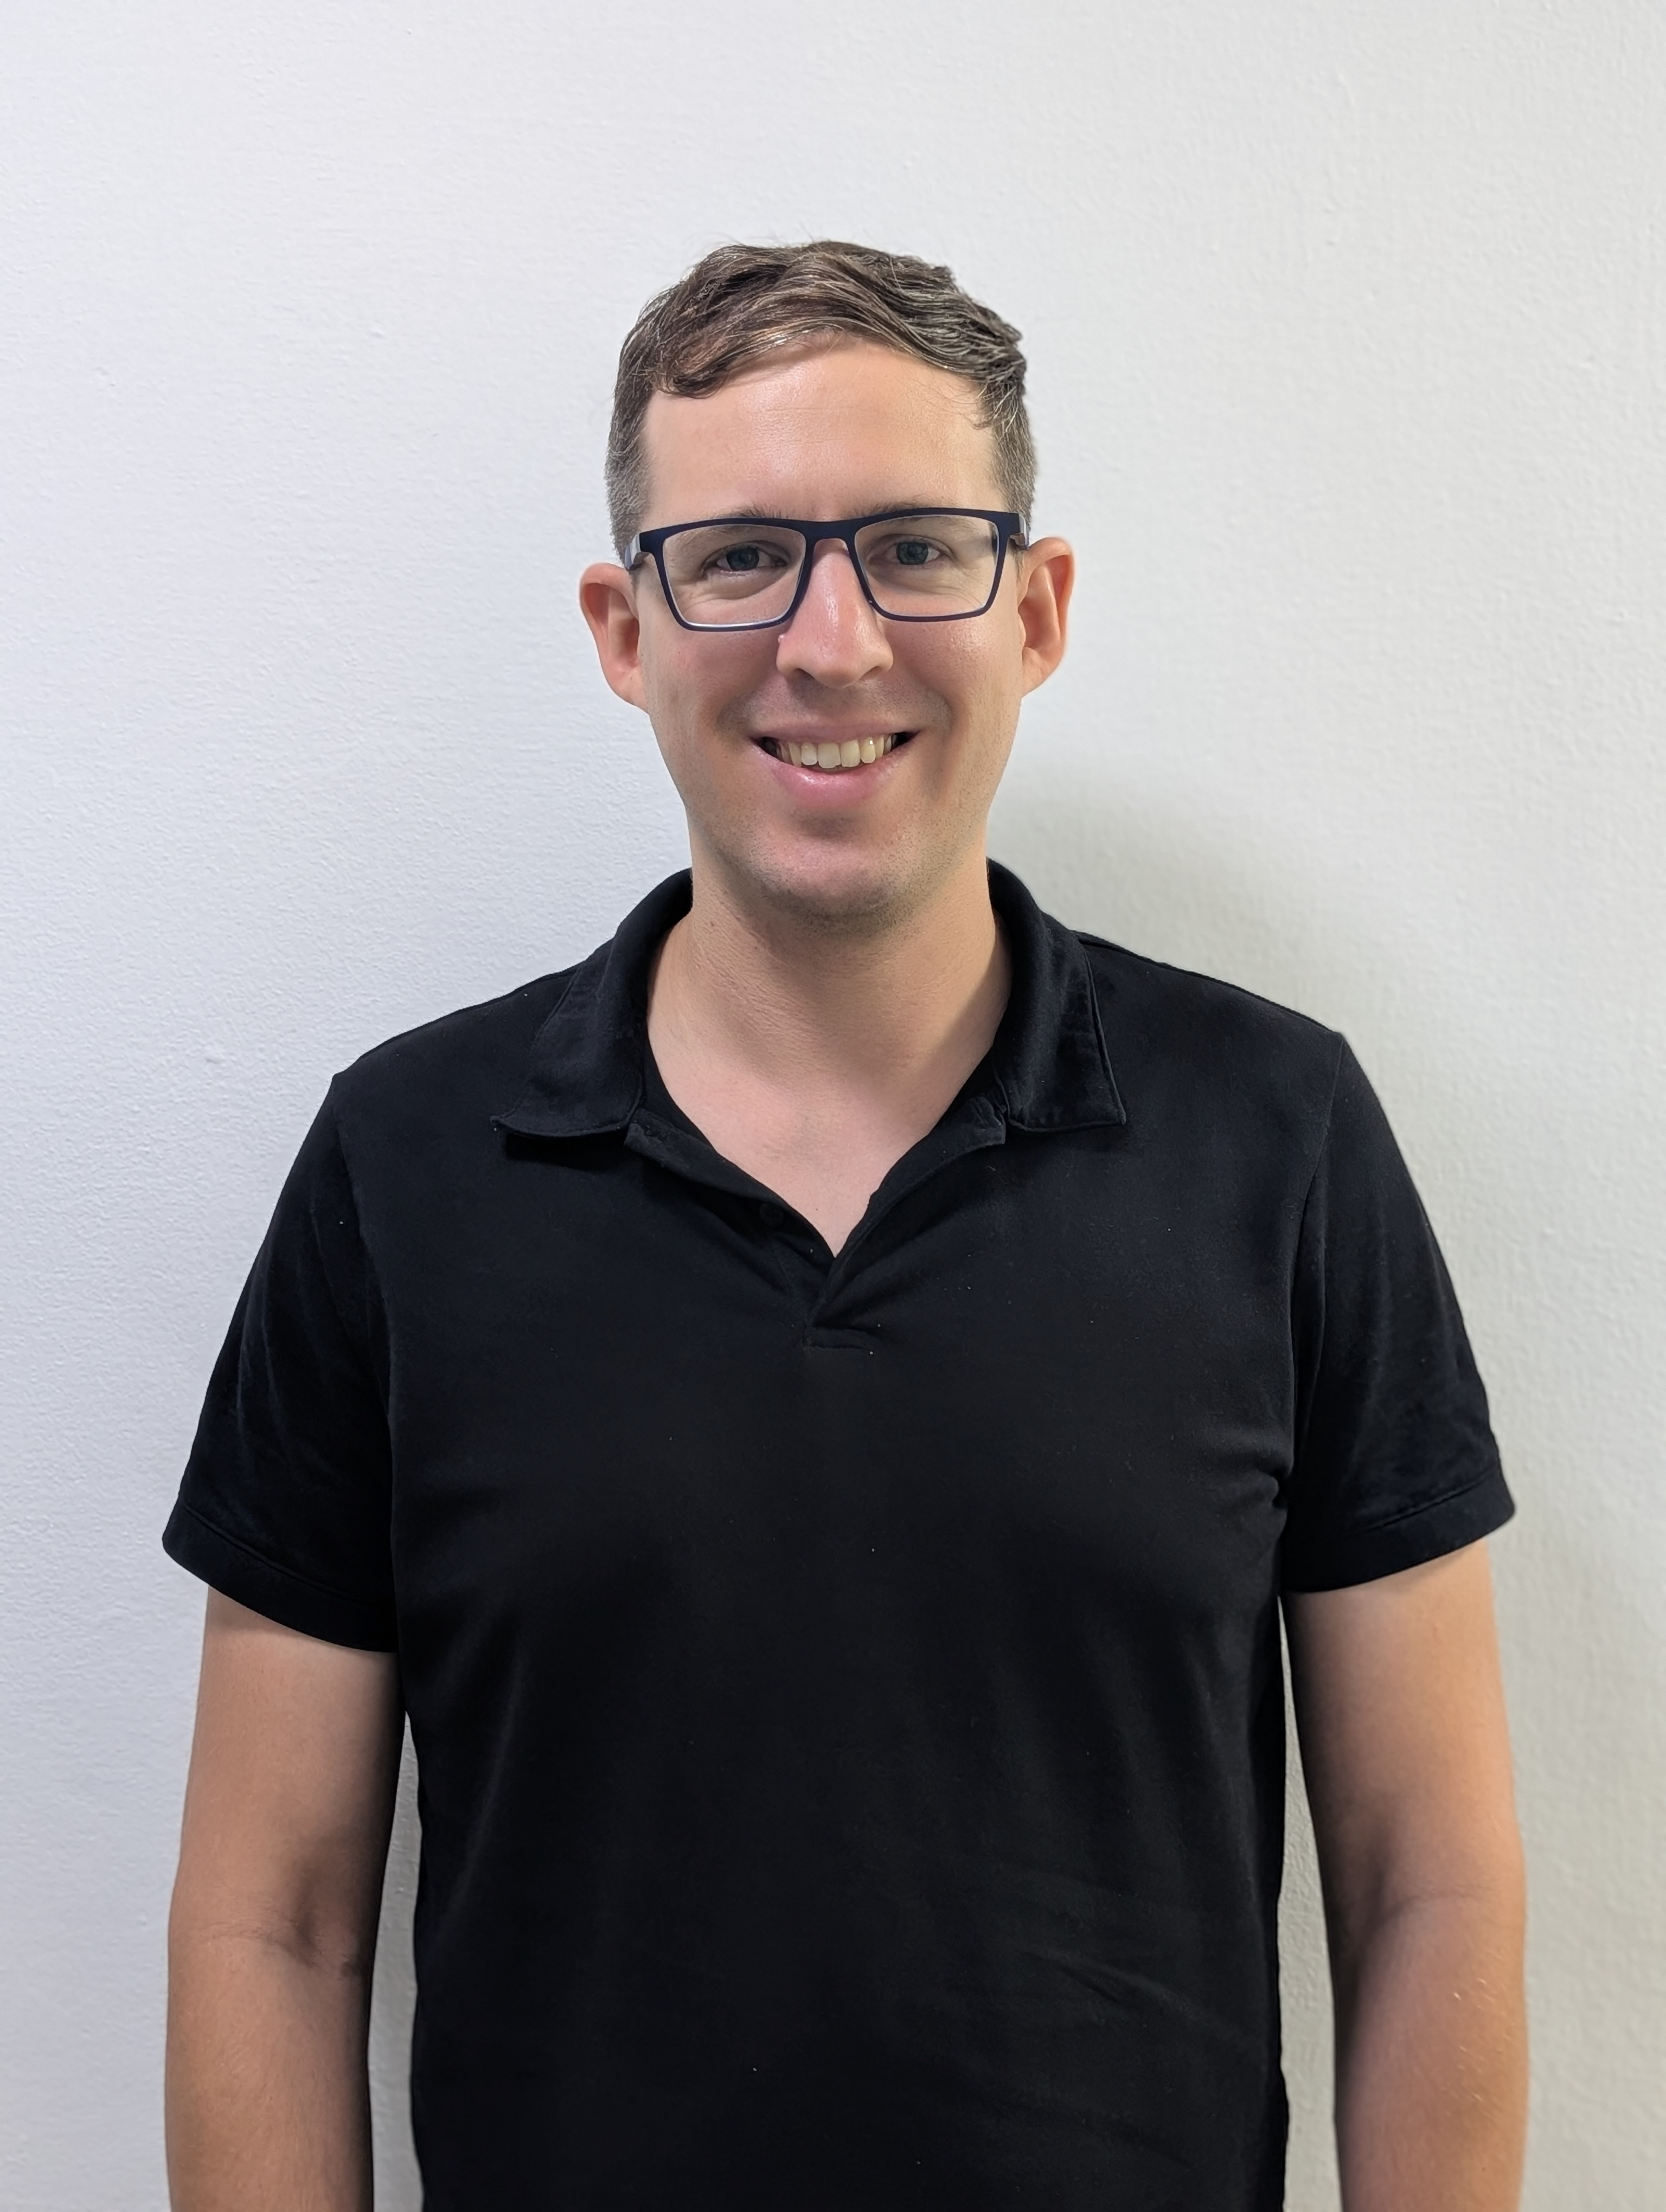
\includegraphics[width=3cm,trim=720bp 1840bp 720bp 250bp,clip]{../Pictures/portrait.jpg}
\end{minipage}

\cvsection{Education}
\datedentry{2022--present}{%
  PhD in Computer Science (in progress), Weizmann Institute of Science.\newline
  Advisor: Prof. Amir Abboud.\newline
  Thesis: \emph{Structure versus Pseudorandomness in Fine-Grained Complexity}.}
\datedentry{2018--2021}{%
  MSc in Computer Science, University of Haifa.\newline
  Advisor: Prof. Oren Weimann.}
\datedentry{2014--2018}{%
  BSc in Computer Science, University of Haifa.}

\cvsection{Professional Experience and Activities}
\datedentry{July 2024}{Teaching Assistant, DIMACS, Rutgers University.}
\datedentry{2017--2021}{%
  Teaching Assistant, Department of Computer Science, University of Haifa.}
\datedentry{2016--2018}{%
  Private tutor, academic support program for BSc students experiencing academic
  difficulties, University of Haifa.}

\textbf{Conference presentations:} ISAAC 2022, ITCS 2023, HALG 2023, ESA 2024,
SODA 2025, ITCS 2026, and HALG 2026.
\par\smallskip
\textbf{Reviewer for:}
\begin{itemize}[leftmargin=*,itemsep=0pt,parsep=0pt,topsep=2pt]
  \item IEEE Symposium on Foundations of Computer Science (FOCS).
  \item ACM-SIAM Symposium on Discrete Algorithms (SODA).
  \item International Colloquium on Automata, Languages, and Programming (ICALP).
  \item Innovations in Theoretical Computer Science Conference (ITCS).
  \item European Symposium on Algorithms (ESA).
  \item Scandinavian Symposium on Algorithm Theory (SWAT).
  \item International Symposium on Mathematical Foundations of Computer Science (MFCS).
  \item Annual Symposium on Combinatorial Pattern Matching (CPM).
\end{itemize}

\cvsection{Teaching and Academic Service}
\datedentry{2022--present}{%
  Algorithms Seminar Organizer, Weizmann Institute of Science.\newline
  Select speakers, coordinate logistics, and host guests.}
\datedentry{July 2024}{DIMACS Tutorial on Fine-Grained Complexity, Rutgers University.}
\datedentry{2018--2021}{Data Structures, University of Haifa.}
\datedentry{2017--2021}{Advanced Data Structures and Probability, University of Haifa.}

\cvsection{Honours and Awards}
\datedentry{2021}{Dean's List, University of Haifa (MSc in Computer Science).}
\datedentry{2019--2020}{Excellence scholarship, University of Haifa.}

\smallskip
{\small\textbf{Languages:} Hebrew, English, French.\par}

\newpage
\cvsection{Publications}
\begin{enumerate}[leftmargin=*,itemsep=0.65\baselineskip,parsep=0pt,topsep=0pt]
  \publication{Lower Bounds for Structured OMv, APSP, and Triangle Detection.}
    {Amir Abboud, Shyan Akmal, Ron Safier, and Nathan Wallheimer.}
    {\emph{Innovations in Theoretical Computer Science Conference (ITCS 2027)}.
    To appear.}

  \publication{Equivalent Dichotomies for Triangle Detection in Subgraph, Induced,
    and Colored H-Free Graphs.}
    {Amir Abboud, Ron Safier, and Nathan Wallheimer.}
    {In \emph{34th Annual European Symposium on Algorithms (ESA 2026)},
    LIPIcs 388, pp.\ 64:1--64:22. Schloss Dagstuhl -- Leibniz-Zentrum f\"ur
    Informatik, 2026. \doi{10.4230/LIPIcs.ESA.2026.64}.}

  \publication{Witness-Sensitive Detection of Induced Diamonds.}
    {Keren Censor-Hillel, Tomer Even, Virginia Vassilevska Williams, and Nathan Wallheimer.}
    {In \emph{53rd International Colloquium on Automata, Languages, and
    Programming (ICALP 2026)}, LIPIcs 374, pp.\ 52:1--52:22.
    Schloss Dagstuhl -- Leibniz-Zentrum f\"ur Informatik, 2026.
    \doi{10.4230/LIPIcs.ICALP.2026.52}.}

  \publication{Triangle Detection in H-Free Graphs.}
    {Amir Abboud, Ron Safier, and Nathan Wallheimer.}
    {In \emph{17th Innovations in Theoretical Computer Science Conference
    (ITCS 2026)}, LIPIcs 362, pp.\ 1:1--1:19.
    Schloss Dagstuhl -- Leibniz-Zentrum f\"ur Informatik, 2026.
    \doi{10.4230/LIPIcs.ITCS.2026.1}.}

  \publication{Recognizing Sumsets is NP-Complete.}
    {Amir Abboud, Nick Fischer, Ron Safier, and Nathan Wallheimer.}
    {In \emph{Proceedings of the 2025 Annual ACM-SIAM Symposium on Discrete
    Algorithms (SODA)}, pp.\ 4484--4506. SIAM, 2025.
    \doi{10.1137/1.9781611978322.153}.}

  \publication{Worst-Case to Expander-Case Reductions: Derandomized and Generalized.}
    {Amir Abboud and Nathan Wallheimer.}
    {In \emph{32nd Annual European Symposium on Algorithms (ESA 2024)},
    LIPIcs 308, pp.\ 4:1--4:18.
    Schloss Dagstuhl -- Leibniz-Zentrum f\"ur Informatik, 2024.
    \doi{10.4230/LIPIcs.ESA.2024.4}.}

  \publication{Worst-Case to Expander-Case Reductions.}
    {Amir Abboud and Nathan Wallheimer.}
    {In \emph{14th Innovations in Theoretical Computer Science Conference
    (ITCS 2023)}, LIPIcs 251, pp.\ 1:1--1:23.
    Schloss Dagstuhl -- Leibniz-Zentrum f\"ur Informatik, 2023.
    \doi{10.4230/LIPIcs.ITCS.2023.1}.}

  \publication{Improved Compression of the Okamura-Seymour Metric.}
    {Shay Mozes, Nathan Wallheimer, and Oren Weimann.}
    {In \emph{33rd International Symposium on Algorithms and Computation
    (ISAAC 2022)}, LIPIcs 248, pp.\ 27:1--27:19.
    Schloss Dagstuhl -- Leibniz-Zentrum f\"ur Informatik, 2022.
    \doi{10.4230/LIPIcs.ISAAC.2022.27}.}
\end{enumerate}

\end{document}
